\documentclass[10pt,a4paper]{article}\usepackage[]{graphicx}\usepackage[]{color}
%% maxwidth is the original width if it is less than linewidth
%% otherwise use linewidth (to make sure the graphics do not exceed the margin)
\makeatletter
\def\maxwidth{ %
  \ifdim\Gin@nat@width>\linewidth
    \linewidth
  \else
    \Gin@nat@width
  \fi
}
\makeatother

\definecolor{fgcolor}{rgb}{0.345, 0.345, 0.345}
\newcommand{\hlnum}[1]{\textcolor[rgb]{0.686,0.059,0.569}{#1}}%
\newcommand{\hlstr}[1]{\textcolor[rgb]{0.192,0.494,0.8}{#1}}%
\newcommand{\hlcom}[1]{\textcolor[rgb]{0.678,0.584,0.686}{\textit{#1}}}%
\newcommand{\hlopt}[1]{\textcolor[rgb]{0,0,0}{#1}}%
\newcommand{\hlstd}[1]{\textcolor[rgb]{0.345,0.345,0.345}{#1}}%
\newcommand{\hlkwa}[1]{\textcolor[rgb]{0.161,0.373,0.58}{\textbf{#1}}}%
\newcommand{\hlkwb}[1]{\textcolor[rgb]{0.69,0.353,0.396}{#1}}%
\newcommand{\hlkwc}[1]{\textcolor[rgb]{0.333,0.667,0.333}{#1}}%
\newcommand{\hlkwd}[1]{\textcolor[rgb]{0.737,0.353,0.396}{\textbf{#1}}}%

\usepackage{framed}
\makeatletter
\newenvironment{kframe}{%
 \def\at@end@of@kframe{}%
 \ifinner\ifhmode%
  \def\at@end@of@kframe{\end{minipage}}%
  \begin{minipage}{\columnwidth}%
 \fi\fi%
 \def\FrameCommand##1{\hskip\@totalleftmargin \hskip-\fboxsep
 \colorbox{shadecolor}{##1}\hskip-\fboxsep
     % There is no \\@totalrightmargin, so:
     \hskip-\linewidth \hskip-\@totalleftmargin \hskip\columnwidth}%
 \MakeFramed {\advance\hsize-\width
   \@totalleftmargin\z@ \linewidth\hsize
   \@setminipage}}%
 {\par\unskip\endMakeFramed%
 \at@end@of@kframe}
\makeatother

\definecolor{shadecolor}{rgb}{.97, .97, .97}
\definecolor{messagecolor}{rgb}{0, 0, 0}
\definecolor{warningcolor}{rgb}{1, 0, 1}
\definecolor{errorcolor}{rgb}{1, 0, 0}
\newenvironment{knitrout}{}{} % an empty environment to be redefined in TeX

\usepackage{alltt}
\usepackage[latin1]{inputenc}
\usepackage{amsmath}
\usepackage{amsfonts}
\usepackage{amssymb}
\author{Erika Martínez}
\title{Guías prácticas}
\IfFileExists{upquote.sty}{\usepackage{upquote}}{}
\begin{document}

\maketitle
\newpage


Crear el vector de datos.
\begin{knitrout}
\definecolor{shadecolor}{rgb}{0.969, 0.969, 0.969}\color{fgcolor}\begin{kframe}
\begin{alltt}
\hlstd{Hijos} \hlkwb{<-} \hlkwd{c}\hlstd{(}\hlnum{2}\hlstd{,} \hlnum{1}\hlstd{)}
\hlkwd{data.entry}\hlstd{(Hijos)}
\hlstd{Hijos}
\end{alltt}
\begin{verbatim}
## [1] 2 1
\end{verbatim}
\begin{alltt}
\hlkwd{length}\hlstd{(Hijos)}
\end{alltt}
\begin{verbatim}
## [1] 2
\end{verbatim}
\end{kframe}
\end{knitrout}


Guardar el vector de datos en un archivo de texto.
\begin{knitrout}
\definecolor{shadecolor}{rgb}{0.969, 0.969, 0.969}\color{fgcolor}\begin{kframe}
\begin{alltt}
\hlkwd{write}\hlstd{(Hijos,} \hlstr{"Hijos.txt"}\hlstd{)}
\end{alltt}
\end{kframe}
\end{knitrout}

Limpiar el área de trabajo (Workspace)
\begin{knitrout}
\definecolor{shadecolor}{rgb}{0.969, 0.969, 0.969}\color{fgcolor}\begin{kframe}
\begin{alltt}
\hlkwd{ls}\hlstd{()}
\end{alltt}
\begin{verbatim}
## [1] "Hijos"
\end{verbatim}
\begin{alltt}
\hlkwd{rm}\hlstd{(}\hlkwc{list}\hlstd{=}\hlkwd{ls}\hlstd{(}\hlkwc{all}\hlstd{=}\hlnum{TRUE}\hlstd{));} \hlkwd{ls}\hlstd{()}
\end{alltt}
\begin{verbatim}
## character(0)
\end{verbatim}
\end{kframe}
\end{knitrout}


Leer o recuperar el vector de datos o archivo de texto
\begin{knitrout}
\definecolor{shadecolor}{rgb}{0.969, 0.969, 0.969}\color{fgcolor}\begin{kframe}
\begin{alltt}
\hlstd{X} \hlkwb{<-} \hlkwd{scan}\hlstd{(}\hlstr{"Hijos.txt"}\hlstd{,} \hlkwc{what} \hlstd{=} \hlkwd{integer}\hlstd{(}\hlnum{0}\hlstd{),} \hlkwc{na.strings} \hlstd{=} \hlstr{"NA"}\hlstd{,} \hlkwc{flush}\hlstd{=}\hlnum{FALSE}\hlstd{)}
\hlkwd{ls}\hlstd{()}
\end{alltt}
\begin{verbatim}
## [1] "X"
\end{verbatim}
\end{kframe}
\end{knitrout}


Gráfico de puntos
\begin{knitrout}
\definecolor{shadecolor}{rgb}{0.969, 0.969, 0.969}\color{fgcolor}\begin{kframe}
\begin{alltt}
\hlkwd{stripchart}\hlstd{(X,} \hlkwc{method}\hlstd{=}\hlstr{"stack"}\hlstd{,} \hlkwc{vertical}\hlstd{=}\hlnum{FALSE}\hlstd{,} \hlkwc{col}\hlstd{=}\hlstr{"blue"}\hlstd{,} \hlkwc{pch}\hlstd{=}\hlnum{1}\hlstd{,} \hlkwc{main}\hlstd{=}\hlstr{"Gráfico de\textbackslash{}n
puntos"}\hlstd{,} \hlkwc{xlab}\hlstd{=}\hlstr{"Número de hijos"}\hlstd{)}
\end{alltt}
\end{kframe}
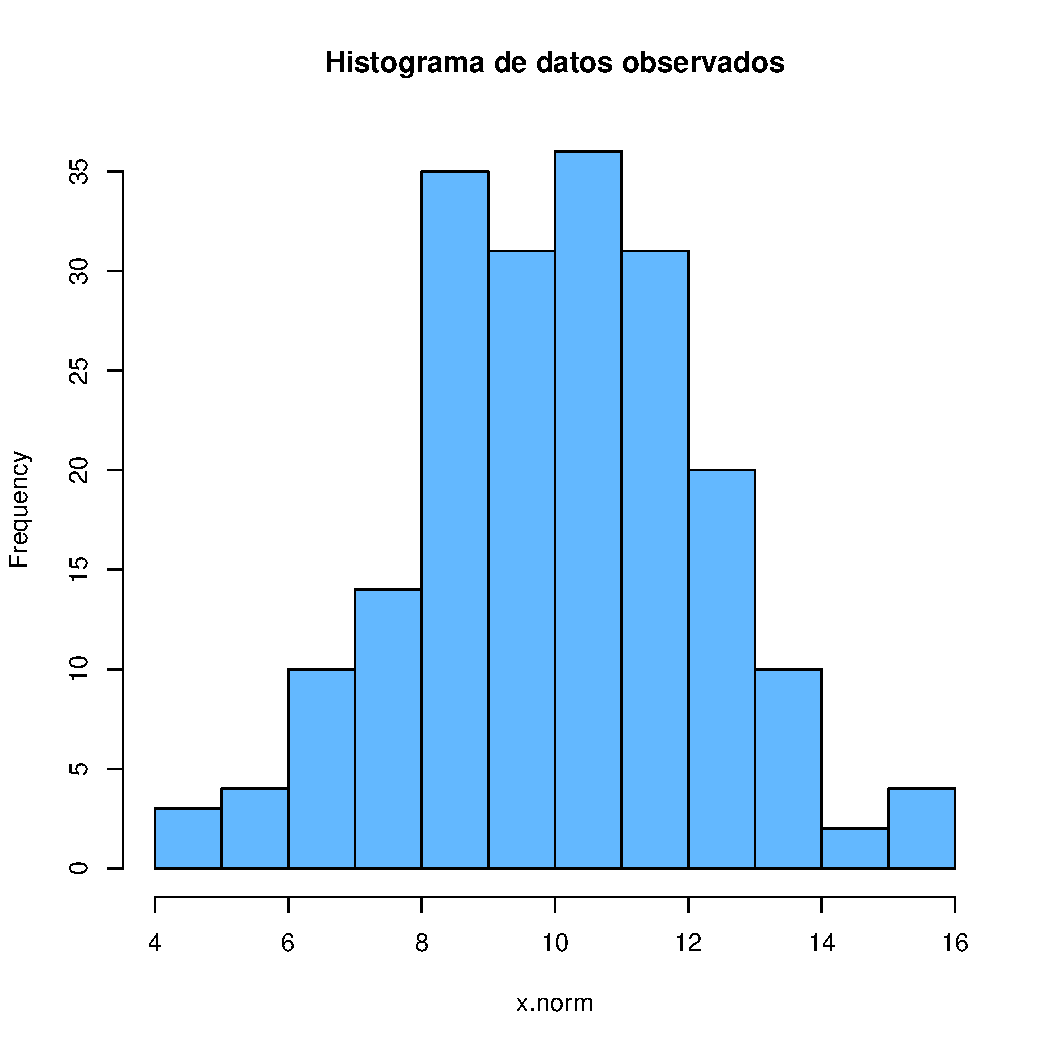
\includegraphics[width=\maxwidth]{figure/unnamed-chunk-5-1} 

\end{knitrout}


 Crear la tabla de frecuencias completa
 frecuencias individuales
\begin{knitrout}
\definecolor{shadecolor}{rgb}{0.969, 0.969, 0.969}\color{fgcolor}\begin{kframe}
\begin{alltt}
\hlstd{fab} \hlkwb{<-} \hlkwd{table}\hlstd{(X); fab} \hlcom{# frecuencias absolutas}
\end{alltt}
\begin{verbatim}
## X
## 1 2 
## 1 1
\end{verbatim}
\begin{alltt}
\hlstd{fre} \hlkwb{<-} \hlstd{fab}\hlopt{/}\hlkwd{length}\hlstd{(X); fre} \hlcom{# frecuencias relativas}
\end{alltt}
\begin{verbatim}
## X
##   1   2 
## 0.5 0.5
\end{verbatim}
\begin{alltt}
\hlstd{Fac} \hlkwb{<-} \hlkwd{cumsum}\hlstd{(fab); Fac} \hlcom{# frecuencias acumuladas}
\end{alltt}
\begin{verbatim}
## 1 2 
## 1 2
\end{verbatim}
\begin{alltt}
\hlstd{Far} \hlkwb{<-} \hlstd{Fac}\hlopt{/}\hlkwd{length}\hlstd{(X); Far} \hlcom{# frecuencias acumuladas relativas}
\end{alltt}
\begin{verbatim}
##   1   2 
## 0.5 1.0
\end{verbatim}
\end{kframe}
\end{knitrout}

 tabla de frecuencias completa
\begin{knitrout}
\definecolor{shadecolor}{rgb}{0.969, 0.969, 0.969}\color{fgcolor}\begin{kframe}
\begin{alltt}
\hlkwd{options}\hlstd{(}\hlkwc{digits}\hlstd{=}\hlnum{2}\hlstd{)}
\hlstd{tabla} \hlkwb{<-} \hlkwd{data.frame}\hlstd{(}\hlkwc{fab}\hlstd{=fab,} \hlkwc{fre}\hlstd{=fre,} \hlkwc{Fac}\hlstd{=Fac,} \hlkwc{Far}\hlstd{=Far)}
\hlkwd{names}\hlstd{(tabla)} \hlkwb{<-} \hlkwd{c}\hlstd{(}\hlstr{"X"}\hlstd{,} \hlstr{"fab"}\hlstd{,} \hlstr{"free.X"}\hlstd{,} \hlstr{"fre"}\hlstd{,} \hlstr{"Fac"}\hlstd{,} \hlstr{"Far"}\hlstd{)}
\hlstd{tabla}
\end{alltt}
\begin{verbatim}
##   X fab free.X fre Fac Far
## 1 1   1      1 0.5   1 0.5
## 2 2   1      2 0.5   2 1.0
\end{verbatim}
\begin{alltt}
\hlstd{tfre} \hlkwb{<-} \hlkwd{data.frame}\hlstd{(}\hlkwc{X}\hlstd{=tabla}\hlopt{$}\hlstd{X,} \hlkwc{fab}\hlstd{=tabla}\hlopt{$}\hlstd{fab,} \hlkwc{fre}\hlstd{=tabla}\hlopt{$}\hlstd{fre,} \hlkwc{Fac}\hlstd{=tabla}\hlopt{$}\hlstd{Fac,} \hlkwc{Far}\hlstd{=tabla}\hlopt{$}\hlstd{Far)}
\hlstd{tfre}
\end{alltt}
\begin{verbatim}
##   X fab fre Fac Far
## 1 1   1 0.5   1 0.5
## 2 2   1 0.5   2 1.0
\end{verbatim}
\end{kframe}
\end{knitrout}

 Calcular los estadísticos descriptivos de la variable
 Estadísticos de tendencia central de los datos
\begin{knitrout}
\definecolor{shadecolor}{rgb}{0.969, 0.969, 0.969}\color{fgcolor}\begin{kframe}
\begin{alltt}
\hlstd{media} \hlkwb{<-} \hlkwd{mean}\hlstd{(X,} \hlkwc{na.rm} \hlstd{=} \hlnum{FALSE}\hlstd{); media}
\end{alltt}
\begin{verbatim}
## [1] 1.5
\end{verbatim}
\begin{alltt}
\hlkwa{for}\hlstd{(i} \hlkwa{in} \hlnum{1}\hlopt{:}\hlkwd{length}\hlstd{(X))} \hlkwa{if} \hlstd{(fab[i]} \hlopt{==} \hlkwd{max}\hlstd{(fab))} \hlkwa{break}\hlstd{()}
\hlstd{moda} \hlkwb{<-} \hlkwd{names}\hlstd{(fab[i]); moda}
\end{alltt}
\begin{verbatim}
## [1] "1"
\end{verbatim}
\begin{alltt}
\hlstd{mediana} \hlkwb{<-} \hlkwd{median}\hlstd{(X); mediana}
\end{alltt}
\begin{verbatim}
## [1] 1.5
\end{verbatim}
\end{kframe}
\end{knitrout}

   Devuelve la cuasivarianza y la cuasivarianza muestral
\begin{knitrout}
\definecolor{shadecolor}{rgb}{0.969, 0.969, 0.969}\color{fgcolor}\begin{kframe}
\begin{alltt}
  \hlstd{cuasivar} \hlkwb{<-} \hlkwd{var}\hlstd{(X); cuasivar}
\end{alltt}
\begin{verbatim}
## [1] 0.5
\end{verbatim}
\begin{alltt}
\hlstd{s} \hlkwb{<-} \hlkwd{sd}\hlstd{(X); s}
\end{alltt}
\begin{verbatim}
## [1] 0.71
\end{verbatim}
\end{kframe}
\end{knitrout}

  Cálculo de Q1, Q2, Q3
\begin{knitrout}
\definecolor{shadecolor}{rgb}{0.969, 0.969, 0.969}\color{fgcolor}\begin{kframe}
\begin{alltt}
  \hlkwd{quantile}\hlstd{(X,}\hlkwd{c}\hlstd{(}\hlnum{0.25}\hlstd{,} \hlnum{0.5}\hlstd{,} \hlnum{0.75}\hlstd{))}
\end{alltt}
\begin{verbatim}
## 25% 50% 75% 
## 1.2 1.5 1.8
\end{verbatim}
\end{kframe}
\end{knitrout}

En general se pueden encontrar cualquier percentil
\begin{knitrout}
\definecolor{shadecolor}{rgb}{0.969, 0.969, 0.969}\color{fgcolor}\begin{kframe}
\begin{alltt}
  \hlkwd{quantile}\hlstd{(X,} \hlnum{0.6}\hlstd{)}
\end{alltt}
\begin{verbatim}
## 60% 
## 1.6
\end{verbatim}
\end{kframe}
\end{knitrout}
  
  Conocer un resumen de los datos
\begin{knitrout}
\definecolor{shadecolor}{rgb}{0.969, 0.969, 0.969}\color{fgcolor}\begin{kframe}
\begin{alltt}
  \hlstd{resumen} \hlkwb{<-} \hlkwd{summary}\hlstd{(X); resumen}
\end{alltt}
\begin{verbatim}
##    Min. 1st Qu.  Median    Mean 3rd Qu.    Max. 
##     1.0     1.2     1.5     1.5     1.8     2.0
\end{verbatim}
\end{kframe}
\end{knitrout}
Min, Q1, Median, Mean, Q3, Max
\begin{knitrout}
\definecolor{shadecolor}{rgb}{0.969, 0.969, 0.969}\color{fgcolor}\begin{kframe}
\begin{alltt}
  \hlkwd{fivenum}\hlstd{(X)}
\end{alltt}
\begin{verbatim}
## [1] 1.0 1.0 1.5 2.0 2.0
\end{verbatim}
\end{kframe}
\end{knitrout}
  
  min, cuartil menor, mediana, cuartil mayor, max

Gráfico de barras (por ser pocos valores)
\begin{knitrout}
\definecolor{shadecolor}{rgb}{0.969, 0.969, 0.969}\color{fgcolor}\begin{kframe}
\begin{alltt}
  \hlkwd{barplot}\hlstd{(tfre[[}\hlnum{2}\hlstd{]],} \hlkwc{main}\hlstd{=}\hlstr{"Gráfico de barras"}\hlstd{,} \hlkwc{xlab}\hlstd{=}\hlstr{"X = Número Hijos\textbackslash{}n"}\hlstd{,} \hlkwc{ylab}\hlstd{=}\hlstr{"frecuencia"}\hlstd{,}
          \hlkwc{col}\hlstd{=}\hlkwd{c}\hlstd{(}\hlstr{"black"}\hlstd{,} \hlstr{"blue"}\hlstd{,} \hlstr{"purple"}\hlstd{,} \hlstr{"white"}\hlstd{,} \hlstr{"cyan"}\hlstd{,} \hlstr{"red"}\hlstd{),} \hlkwc{sub}\hlstd{=}\hlstr{"Agosto-2012"}\hlstd{)}
\end{alltt}
\end{kframe}
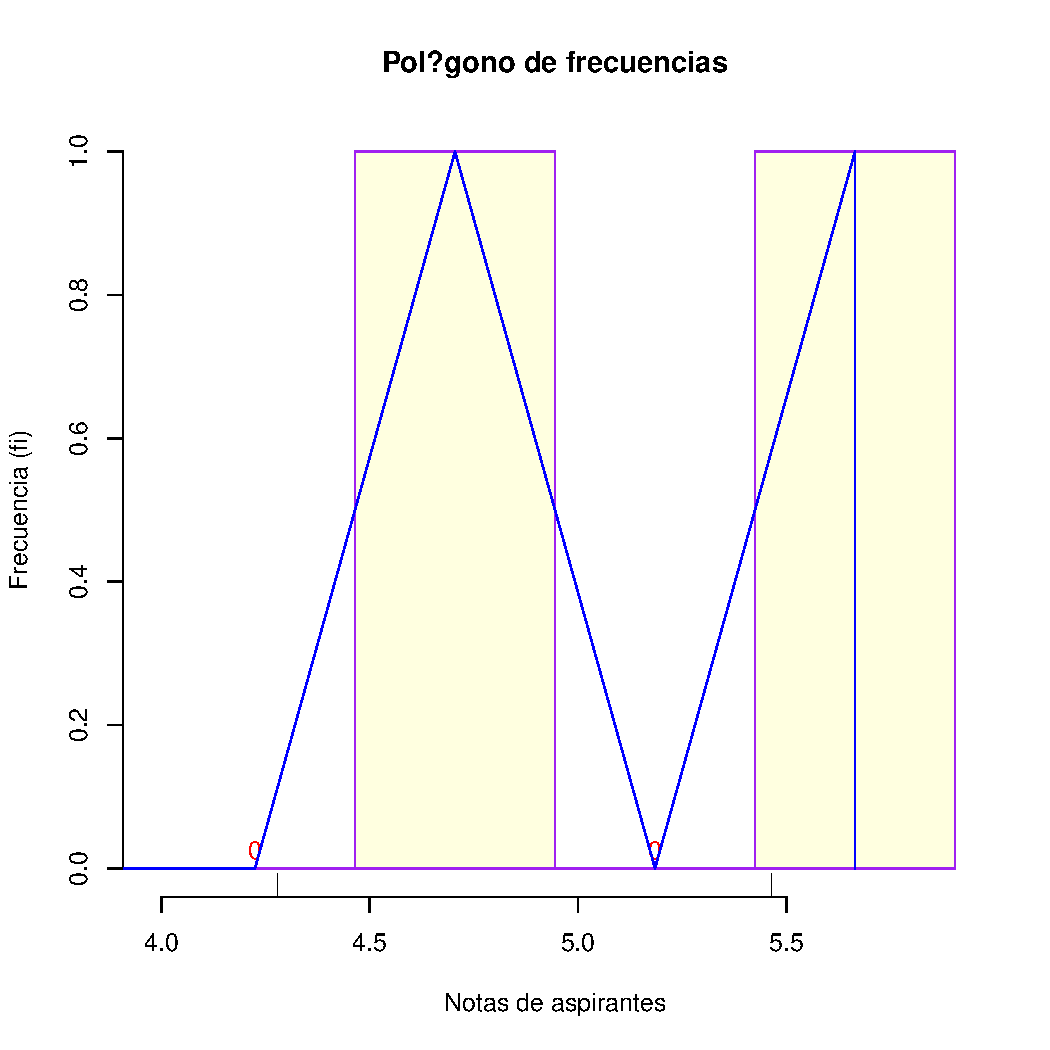
\includegraphics[width=\maxwidth]{figure/unnamed-chunk-14-1} 

\end{knitrout}
  
   Gráfico de pastel (por ser pocos valores)

\begin{knitrout}
\definecolor{shadecolor}{rgb}{0.969, 0.969, 0.969}\color{fgcolor}\begin{kframe}
\begin{alltt}
  \hlkwd{pie}\hlstd{(tfre[[}\hlnum{2}\hlstd{]],} \hlkwc{main}\hlstd{=}\hlstr{"Gráfico de pastel"}\hlstd{,} \hlkwc{xlab}\hlstd{=}\hlstr{"Número Hijos \textbackslash{}n"}\hlstd{,}
      \hlkwc{col}\hlstd{=}\hlkwd{c}\hlstd{(}\hlstr{"black"}\hlstd{,} \hlstr{"blue"}\hlstd{,} \hlstr{"purple"}\hlstd{,} \hlstr{"white"}\hlstd{,} \hlstr{"cyan"}\hlstd{,} \hlstr{"red"}\hlstd{),} \hlkwc{sub}\hlstd{=}\hlstr{"Agosto-2012"}\hlstd{)}
\end{alltt}
\end{kframe}
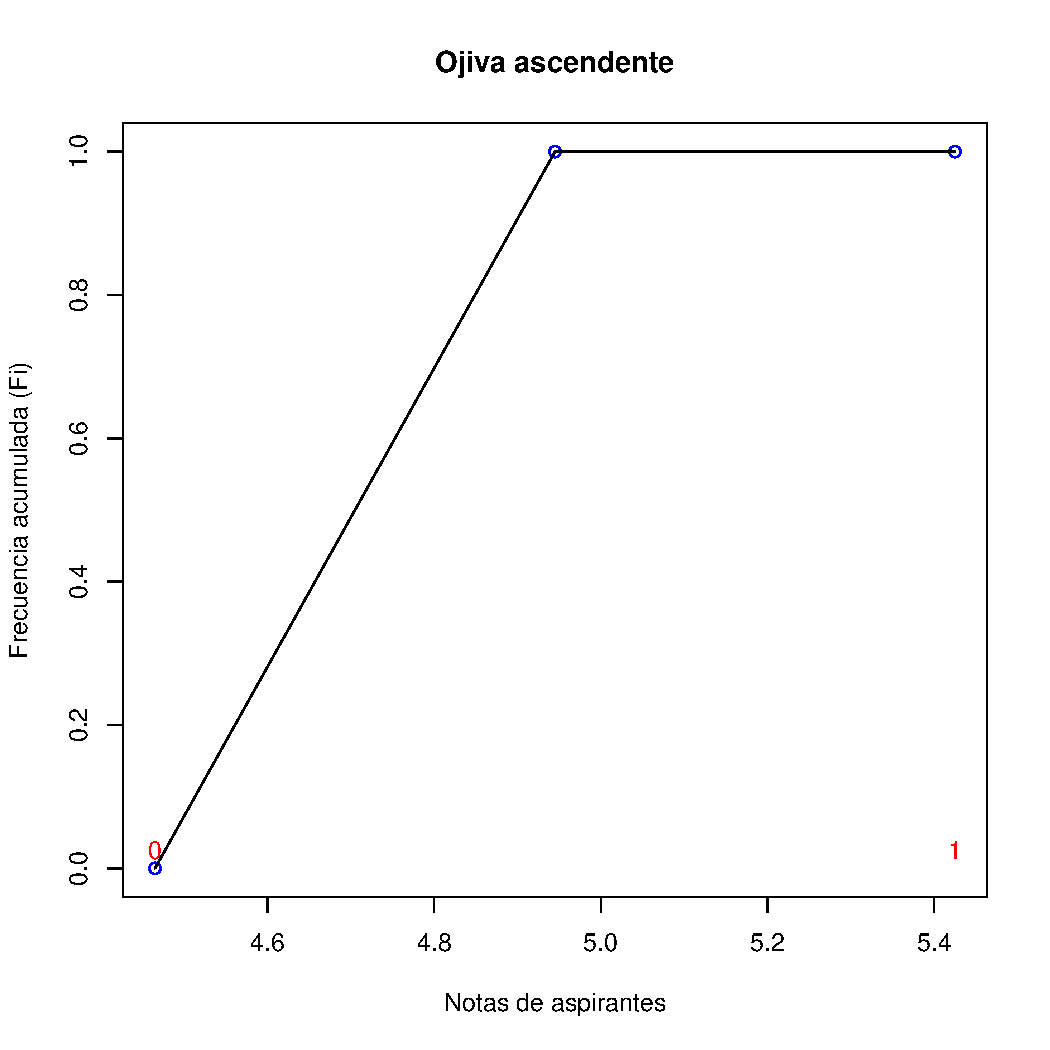
\includegraphics[width=\maxwidth]{figure/unnamed-chunk-15-1} 

\end{knitrout}
  
  
  Se puede especificar nombres para las categorías
\begin{knitrout}
\definecolor{shadecolor}{rgb}{0.969, 0.969, 0.969}\color{fgcolor}\begin{kframe}
\begin{alltt}
  \hlkwd{names}\hlstd{(fab)} \hlkwb{=} \hlkwd{c}\hlstd{(}\hlstr{"Cero"}\hlstd{,} \hlstr{"Uno"}\hlstd{,} \hlstr{"Dos"}\hlstd{,} \hlstr{"Tres"}\hlstd{,} \hlstr{"Cuatro"}\hlstd{,} \hlstr{"Cinco"}\hlstd{)}
\end{alltt}


{\ttfamily\noindent\bfseries\color{errorcolor}{\#\# Error in names(fab) = c("{}Cero"{}, "{}Uno"{}, "{}Dos"{}, "{}Tres"{}, "{}Cuatro"{}, "{}Cinco"{}): el atributo 'names' [6] debe tener la misma longitud que el vector [2]}}\begin{alltt}
\hlkwd{pie}\hlstd{(fab,} \hlkwc{main}\hlstd{=}\hlstr{"Gráfico de pastel"}\hlstd{,} \hlkwc{xlab}\hlstd{=}\hlstr{"X = Número Hijos\textbackslash{}n"}\hlstd{,} \hlkwc{col}\hlstd{=}\hlkwd{c}\hlstd{(}\hlstr{"black"}\hlstd{,} \hlstr{"blue"}\hlstd{,}
                                                                    \hlstr{"purple"}\hlstd{,} \hlstr{"white"}\hlstd{,} \hlstr{"cyan"}\hlstd{,} \hlstr{"red"}\hlstd{),} \hlkwc{sub}\hlstd{=}\hlstr{"Agosto-2012"}\hlstd{)}
\end{alltt}
\end{kframe}
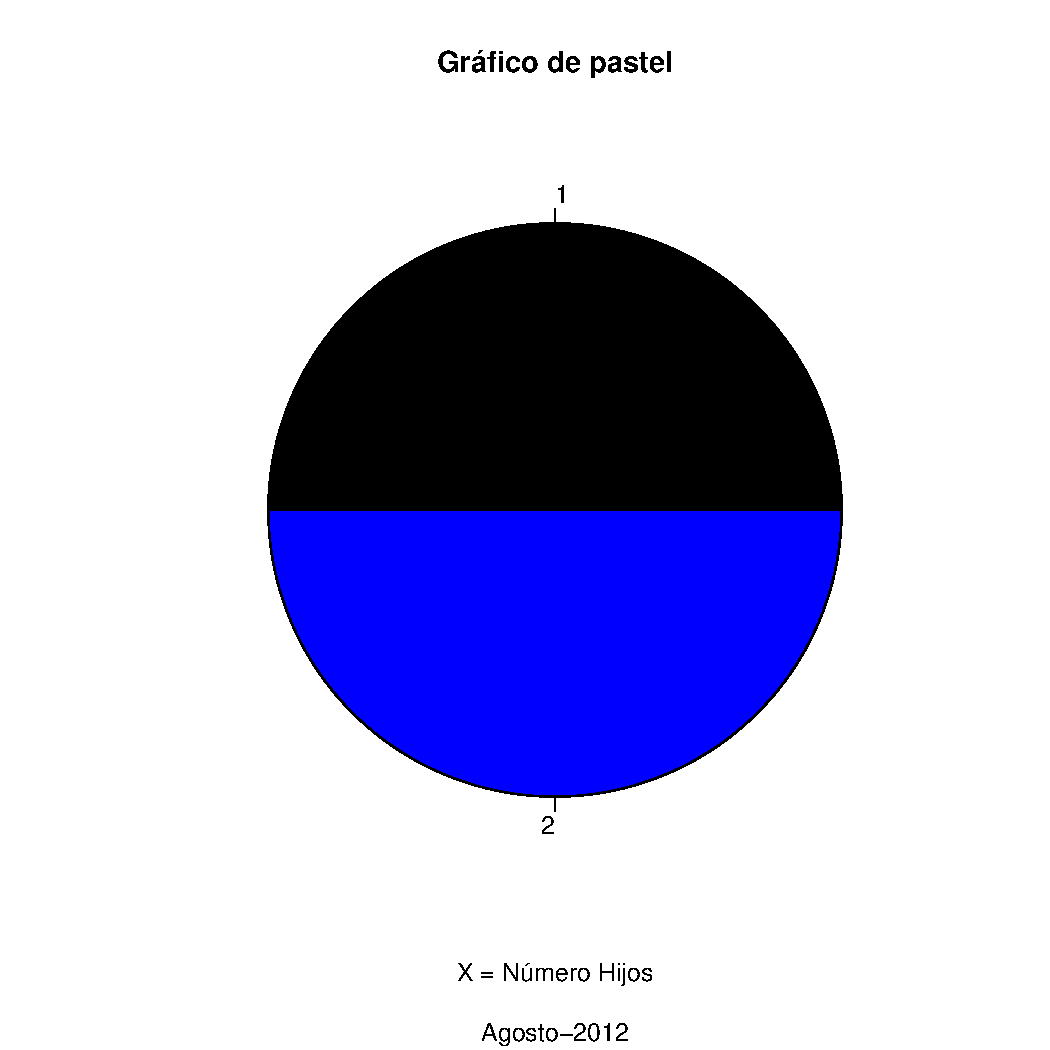
\includegraphics[width=\maxwidth]{figure/unnamed-chunk-16-1} 

\end{knitrout}
 
 
  
  Vertical

\begin{knitrout}
\definecolor{shadecolor}{rgb}{0.969, 0.969, 0.969}\color{fgcolor}\begin{kframe}
\begin{alltt}
  \hlkwd{boxplot}\hlstd{(X,} \hlkwc{main}\hlstd{=}\hlstr{"Gráfico de caja"}\hlstd{,} \hlkwc{xlab}\hlstd{=}\hlstr{" Número de hijos\textbackslash{}n"}\hlstd{,}
          \hlkwc{plot}\hlstd{=}\hlnum{TRUE}\hlstd{,} \hlkwc{border}\hlstd{=}\hlstr{"blue"}\hlstd{,}\hlkwc{col}\hlstd{=}\hlstr{"cyan"}\hlstd{,} \hlkwc{horizontal}\hlstd{=}\hlnum{TRUE}\hlstd{)}
\end{alltt}
\end{kframe}
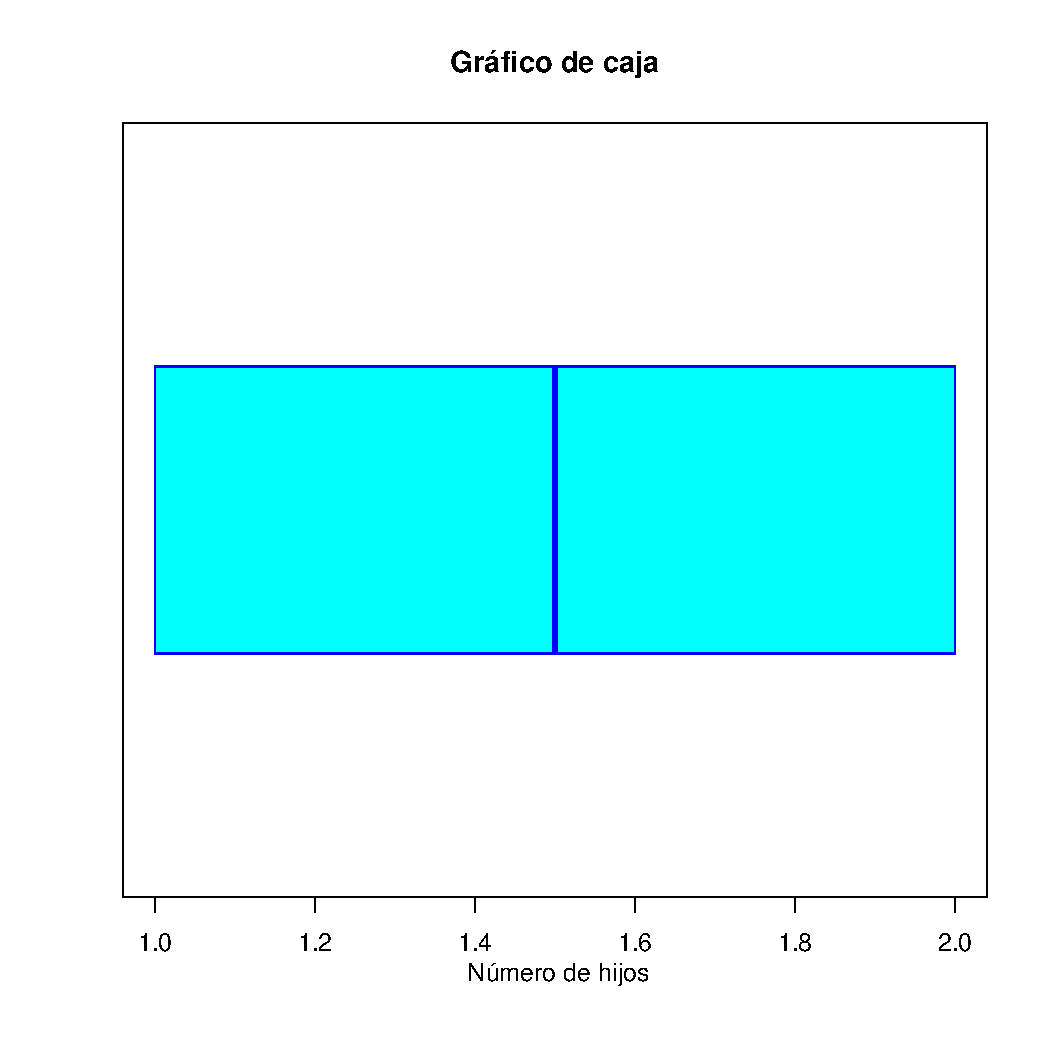
\includegraphics[width=\maxwidth]{figure/unnamed-chunk-17-1} 

\end{knitrout}
 

\end{document}
